In diesem Schritt wollen wir nun die Untersuchungen aus 
\nameref{ch:Content2:sec:a Posteriori} durchführen. Nach dem Rendern eines
$Frames_{t}$(vor dem Rendern von $Frame_{t+1}$) approximieren wir das Histogramm
der Pixelwerte anhand der Pixelwerte von $Frame_{t}$. Dabei betrachten wir
eine Anzahl Pixel pro BLOCK(=16 nach \cite{hal02158423}) in der unmittelbaren Nachbarschaft 
und nehmen diese wie anfangs erwähnt als Schätzung des Histogramms.

\cite{hal02158423}
\begin{algorithm}[H]
    \caption{\textbf{Sortier Schritt t} nach dem Rendern von Frame t
    und vor dem Rendern von Frame t+1}
    \begin{algorithmic}[1]
        \State pixel \textbf{consists of} value,index;
        \State List framePixelsIntensities, noiseIntensities;
        \State $assert(sizeof(framePixelsIntensities)==BLOCKSIZE)$;
        \State $assert(sizeof(noiseIntensities)==BLOCKSIZE)$;
        \State List L $\leftarrow$ pixels of frame t in block;
        \State \hfill
        \State //init lists
        \State initList(framePixelsIntensities, pixelIntensity(L);
        \State $blueNoise_{t}$ = calcCorrectOffset(incomingbluenoisetexture);
        \State initList(noiseIntensities, pixelIntensity($blueNoise_{t}$));
        \State \hfill
        \State //sort the two lists by means of intensities
        \State sort(framePixelsIntensities);
        \State Sort(noiseIntensities);
        \State \hfill
        \State //now we reorder our seeds hence the sorted lists
        \For{$i = 1 .. BLOCKSIZE$}
        \State $sortedSeeds(noiseIntensities.getIndex(i)) = incomingSeeds(framePixelIntensities.getIndex(i))$;
        \EndFor
    \end{algorithmic}
    \label{alg:Sortier}
\end{algorithm}

Hierbei muss noch eine wichtige Anmerkung gemacht werden. Die Fehlerverteilung
der Pixelwerte im Bildraum konvergiert auf diese Weise nicht zu einer 
blue noise Verteilung, denn wir wechseln in jedem Frame die 
verwendeten blue noise Texturen(theoretisch! praktischerweise werden wir hier eine
Textur verwenden und mit Erkenntnissen aus \nameref{ch:Content1:sec:Quasi-Zufallsfolgen}) 
quasi-zufällig zugreifen um so einen solchen Effekt zu erreichen). 
Dieser Schritt alleine reicht also nicht für den erwünschten Effekt zu erreichen.


Die APosteriori Erkenntnisse zu der inversen Funktion\ref{eq:inverse Funktion} garantieren uns nach dem
Umsortieren die entsprechenden Seeds in einer ebenfalls blue noise verteilten Struktur zu erhalten.  

\newpage

\begin{figure}[H]

    \begin{subfigure}{\textwidth}
        \centering 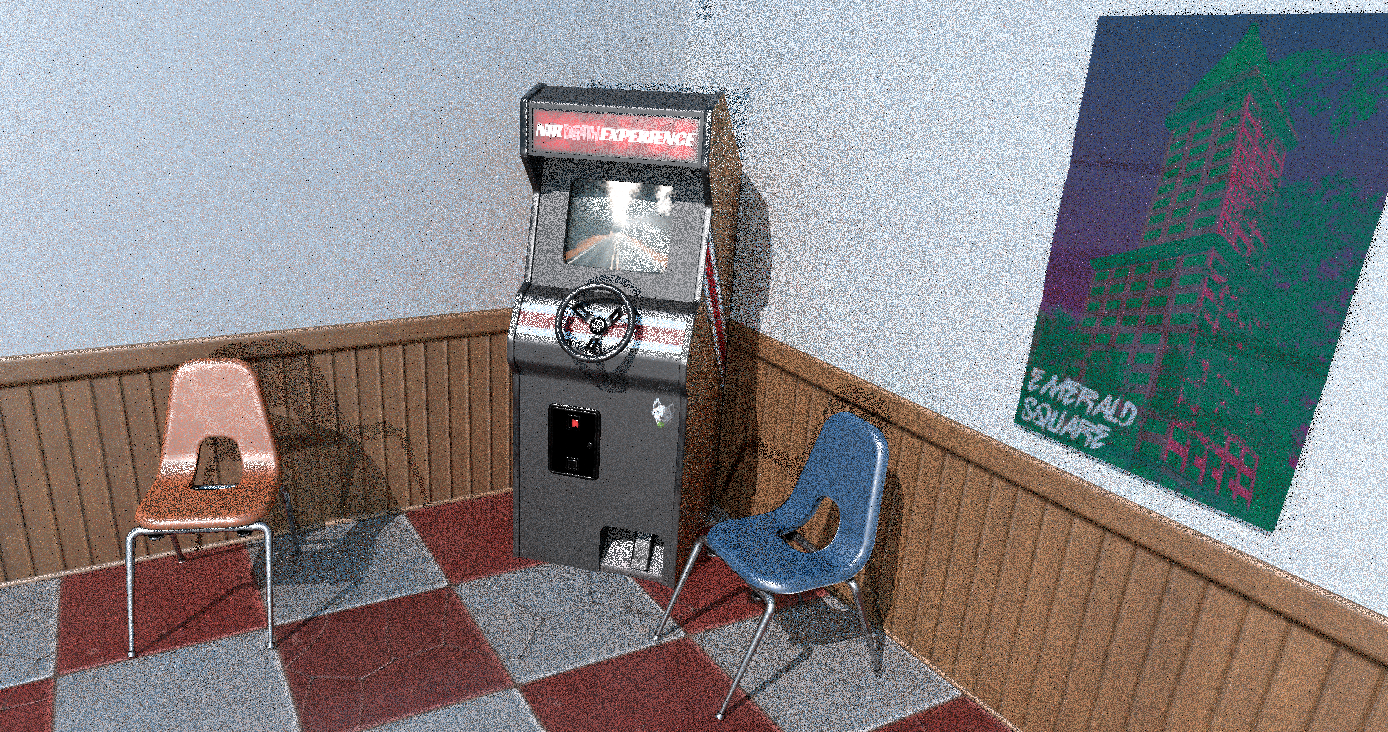
\includegraphics[scale=.25]{content/TemporalerAlg/Bilder/Sorting/Screenshots/seed_debug_3.0_selection.png}
        \caption{Szene}
        \label{fig:Nur_Sorting_Szene_t1}
    \end{subfigure}
    \begin{subfigure}{0.5\textwidth}
        \centering 
\includegraphics[width=0.4\linewidth]{content/TemporalerAlg/Bilder/Sorting/Screenshots/seed_debug_3.0_ausschnitt.png} 
        \caption{Szenenausschnitt}
        \label{fig:Nur_Sorting_ausschnitt_t1}
    \end{subfigure}
    \begin{subfigure}{0.5\textwidth}
        \centering 
\includegraphics[width=0.4\linewidth]{content/TemporalerAlg/Bilder/Sorting/Screenshots/Spektren/seed_debug_3.0_ausschnitt.png}
        \caption{Fouriertransformierte des Ausschnitts}
        \label{fig:Nur_Sorting_Fouriertransformierte_t1}
    \end{subfigure}
        \caption{Zeitpunkt t=1}
        \label{fig:Nur_Sorting_Verlauf_t1}
\end{figure}

\begin{figure}[H]
    \begin{subfigure}{\textwidth}
        \centering 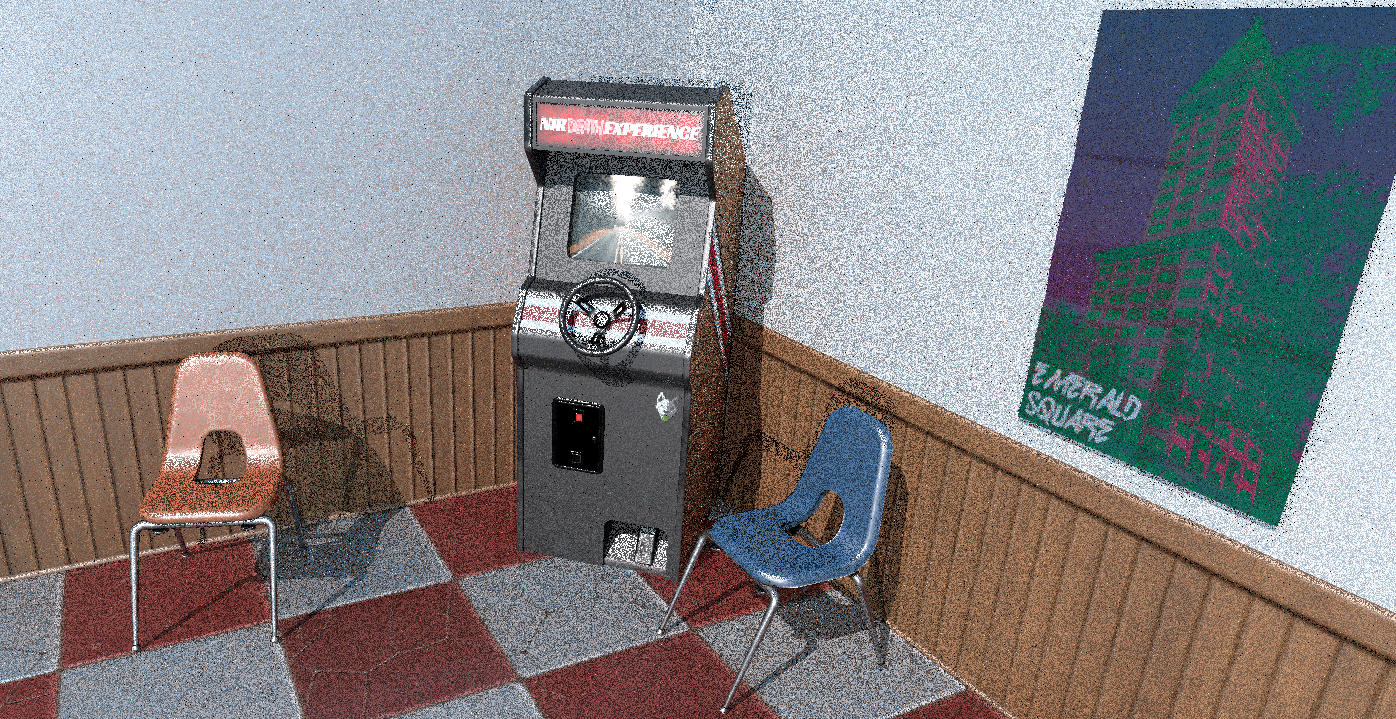
\includegraphics[scale=.25]{content/TemporalerAlg/Bilder/Sorting/Screenshots/seed_debug_4.0_selection.png}
        \caption{Szene}
        \label{fig:Nur_Sorting_Szene_t2}
    \end{subfigure}
    \begin{subfigure}{0.5\textwidth}
        \centering
\includegraphics[width=0.4\linewidth]{content/TemporalerAlg/Bilder/Sorting/Screenshots/seed_debug_4.0_ausschnitt.png} 
        \caption{Szenenausschnitt}
        \label{fig:Nur_Sorting_ausschnitt_t2}
    \end{subfigure}
    \begin{subfigure}{0.5\textwidth}
        \centering
\includegraphics[width=0.4\linewidth]{content/TemporalerAlg/Bilder/Sorting/Screenshots/Spektren/seed_debug_4.0_ausschnitt.png}
        \caption{Fouriertransformierte des Ausschnitts}
        \label{fig:Nur_Sorting_Fouriertransformierte_t2}
    \end{subfigure}
        \caption{Zeitpunkt t=2}
        \label{fig:Nur_Sorting_Verlauf_t2}
\end{figure}

\begin{figure}[H]
    \begin{subfigure}{\textwidth}
        \centering 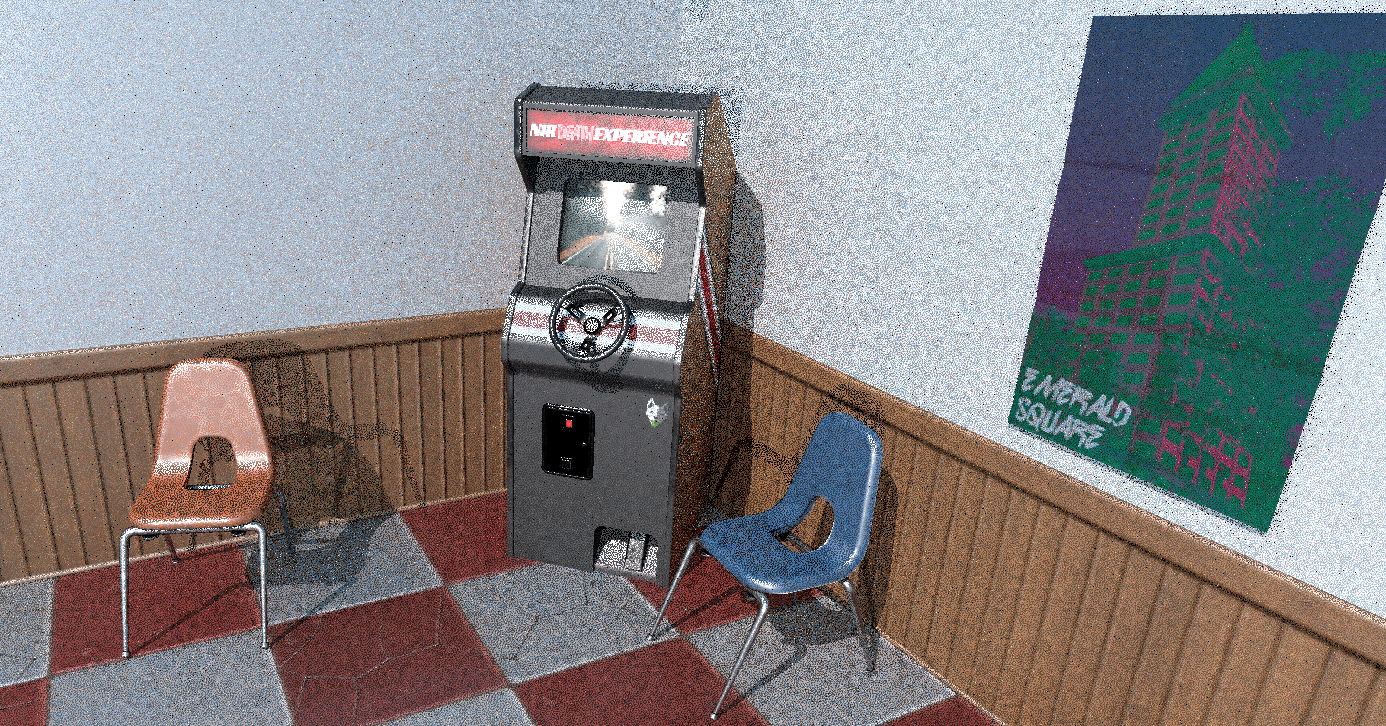
\includegraphics[scale=.25]{content/TemporalerAlg/Bilder/Sorting/Screenshots/seed_debug_5.0_selection.png}
        \caption{Szene}
        \label{fig:Nur_Sorting_Szene_t3}
    \end{subfigure}
    \begin{subfigure}{0.5\textwidth}
        \centering
\includegraphics[width=0.4\linewidth]{content/TemporalerAlg/Bilder/Sorting/Screenshots/seed_debug_5.0_ausschnitt.png} 
        \caption{Szenenausschnitt}
        \label{fig:Nur_Sorting_ausschnitt_t3}
    \end{subfigure}
    \begin{subfigure}{0.5\textwidth}
        \centering
\includegraphics[width=0.4\linewidth]{content/TemporalerAlg/Bilder/Sorting/Screenshots/Spektren/seed_debug_5.0_ausschnitt.png}
        \caption{Fouriertransformierte des Ausschnitts}
        \label{fig:Nur_Sorting_Fouriertransformierte_t3}
    \end{subfigure}
        \caption{Zeitpunkt t=3}
        \label{fig:Nur_Sorting_Verlauf_t3}
\end{figure}

\begin{figure}[H]
    \begin{subfigure}{\textwidth}  
        \centering 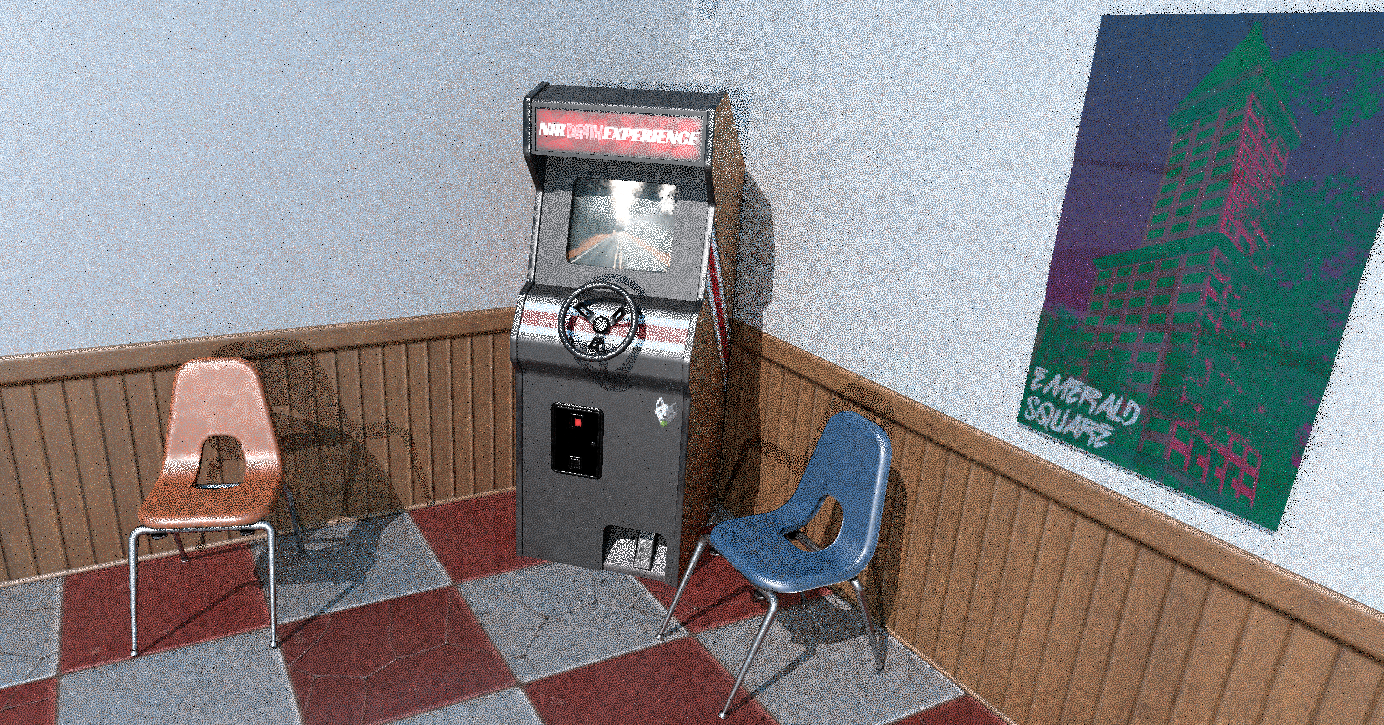
\includegraphics[scale=.25]{content/TemporalerAlg/Bilder/Sorting/Screenshots/seed_debug_6.0_selection.png}
        \caption{Szene}
        \label{fig:Nur_Sorting_Szene_t4}
    \end{subfigure}
    \begin{subfigure}{0.5\textwidth}
        \centering
\includegraphics[width=0.4\linewidth]{content/TemporalerAlg/Bilder/Sorting/Screenshots/seed_debug_6.0_ausschnitt.png} 
        \caption{Szenenausschnitt}
        \label{fig:Nur_Sorting_ausschnitt_t4}
    \end{subfigure}
    \begin{subfigure}{0.5\textwidth}
        \centering
\includegraphics[width=0.4\linewidth]{content/TemporalerAlg/Bilder/Sorting/Screenshots/Spektren/seed_debug_6.0_ausschnitt.png}
        \caption{Fouriertransformierte des Ausschnitts}
        \label{fig:Nur_Sorting_Fouriertransformierte_t4}
    \end{subfigure}
        \caption{Zeitpunkt t=4}
        \label{fig:Nur_Sorting_Verlauf_t4}
\end{figure}

\begin{figure}[H]
    \begin{subfigure}{\textwidth}   
        \centering 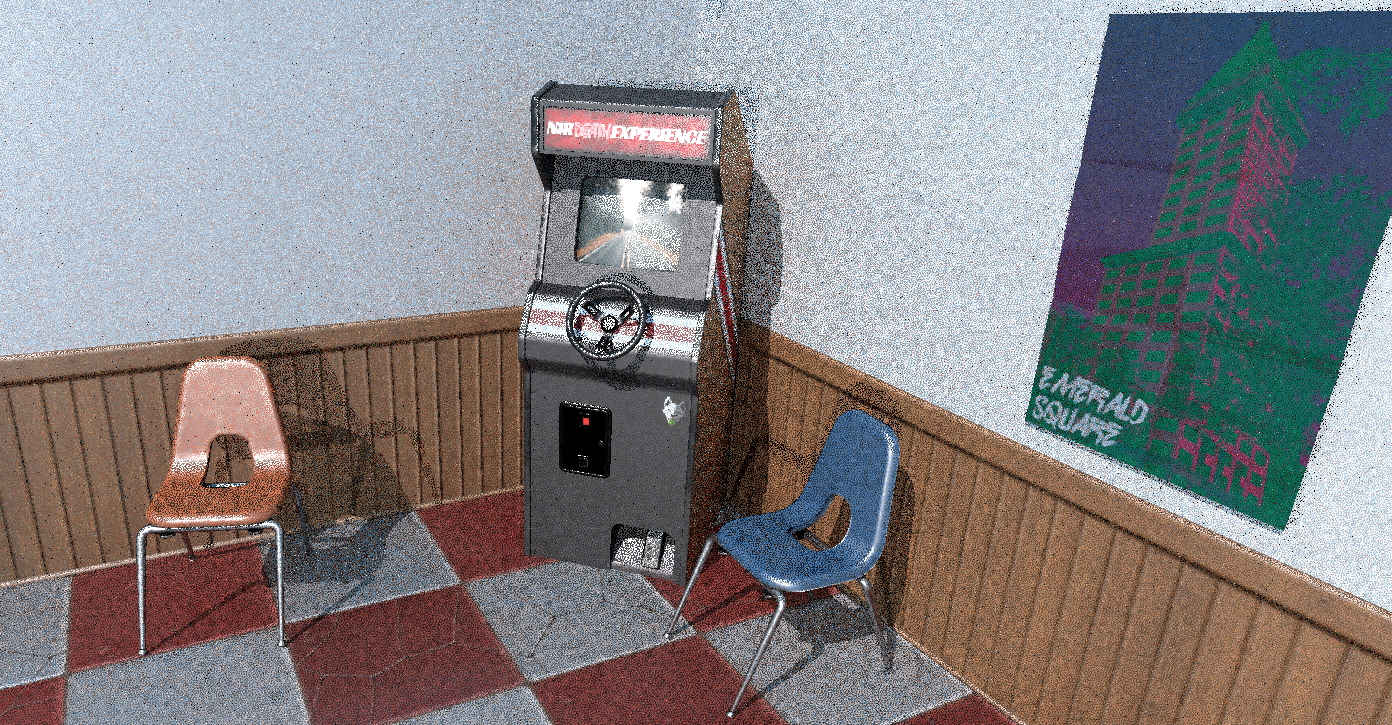
\includegraphics[scale=.25]{content/TemporalerAlg/Bilder/Sorting/Screenshots/seed_debug_7.0_selection.png}
        \caption{Szene}
        \label{fig:Nur_Sorting_Szene_t5}
    \end{subfigure}
    \begin{subfigure}{0.5\textwidth}
        \centering
\includegraphics[width=0.4\linewidth]{content/TemporalerAlg/Bilder/Sorting/Screenshots/seed_debug_7.0_ausschnitt.png} 
        \caption{Szenenausschnitt}
        \label{fig:Nur_Sorting_ausschnitt_t5}
    \end{subfigure}
    \begin{subfigure}{0.5\textwidth}
        \centering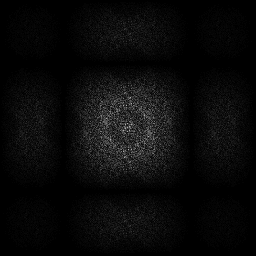
\includegraphics[width=0.4\linewidth]{content/TemporalerAlg/Bilder/Sorting/Screenshots/Spektren/seed_debug_7.0_ausschnitt.png}
        \caption{Fouriertransformierte des Ausschnitts}
        \label{fig:Nur_Sorting_Fouriertransformierte_t5}
    \end{subfigure}
        \caption{Zeitpunkt t=5}
        \label{fig:Nur_Sorting_Verlauf_t5}
\end{figure}

\begin{figure}[H]
    \begin{subfigure}{\textwidth}   
        \centering 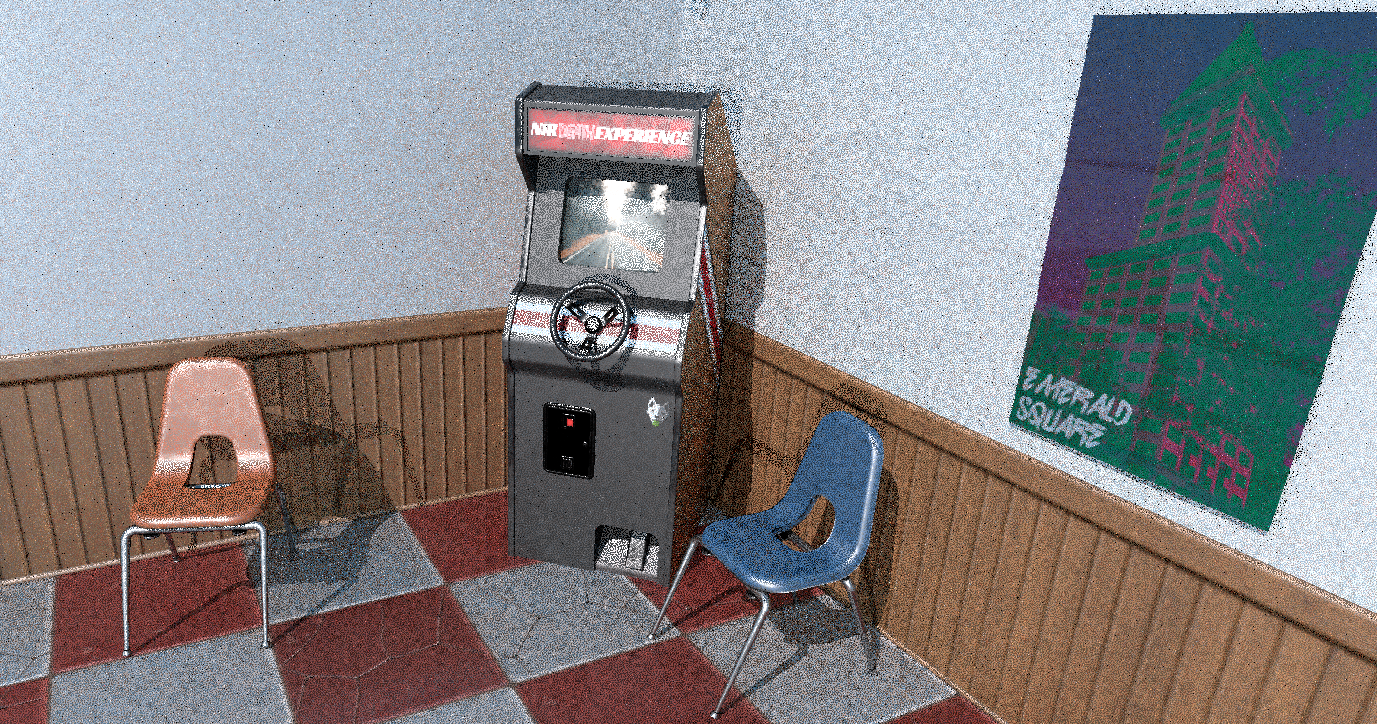
\includegraphics[scale=.25]{content/TemporalerAlg/Bilder/Sorting/Screenshots/seed_debug_8.0_selection.png}
        \caption{Szene}
        \label{fig:Nur_Sorting_Szene_t6}
    \end{subfigure}
    \begin{subfigure}{0.5\textwidth}
        \centering
\includegraphics[width=0.4\linewidth]{content/TemporalerAlg/Bilder/Sorting/Screenshots/seed_debug_8.0_ausschnitt.png} 
        \caption{Szenenausschnitt}
        \label{fig:Nur_Sorting_ausschnitt_t6}
    \end{subfigure}
    \begin{subfigure}{0.5\textwidth}
        \centering
\includegraphics[width=0.4\linewidth]{content/TemporalerAlg/Bilder/Sorting/Screenshots/Spektren/seed_debug_8.0_ausschnitt.png}
        \caption{Fouriertransformierte des Ausschnitts}
        \label{fig:Nur_Sorting_Fouriertransformierte_t6}
    \end{subfigure}
        \caption{Zeitpunkt t=5}
        \label{fig:Nur_Sorting_Verlauf_t6}
\end{figure}

\begin{figure}[H]
    \begin{subfigure}{\textwidth}   
        \centering 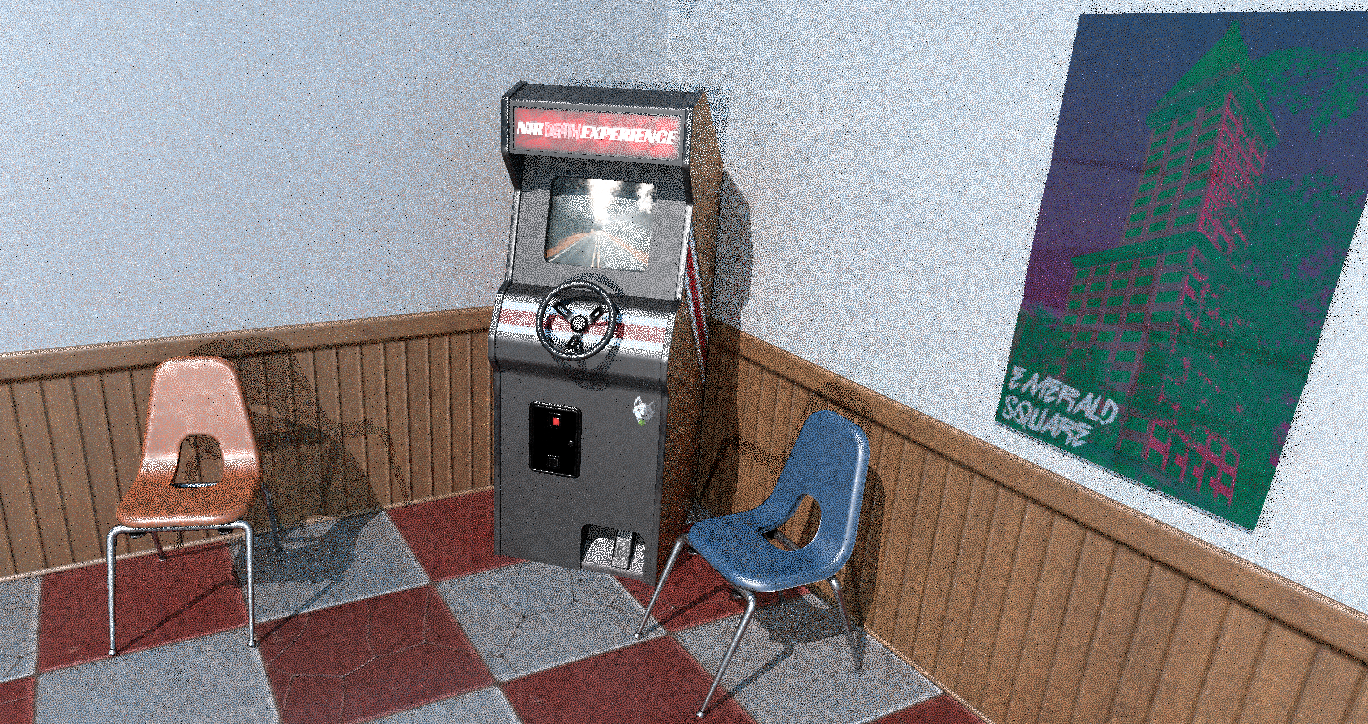
\includegraphics[scale=.25]{content/TemporalerAlg/Bilder/Sorting/Screenshots/seed_debug_9.0_selection.png}
        \caption{Szene}
        \label{fig:Nur_Sorting_Szene_t7}
    \end{subfigure}
    \begin{subfigure}{0.5\textwidth}
        \centering
\includegraphics[width=0.4\linewidth]{content/TemporalerAlg/Bilder/Sorting/Screenshots/seed_debug_9.0_ausschnitt.png} 
        \caption{Szenenausschnitt}
        \label{fig:Nur_Sorting_ausschnitt_t7}
    \end{subfigure}
    \begin{subfigure}{0.5\textwidth}
        \centering
\includegraphics[width=0.4\linewidth]{content/TemporalerAlg/Bilder/Sorting/Screenshots/Spektren/seed_debug_9.0_ausschnitt.png}
        \caption{Fouriertransformierte des Ausschnitts}
        \label{fig:Nur_Sorting_Fouriertransformierte_t7}
    \end{subfigure}
        \caption{Zeitpunkt t=5}
        \label{fig:Nur_Sorting_Verlauf_t7}
\end{figure}